% stumps.tex
% Jeremy Barnes, 22/9/1999
% $Id$

\chapter{Decision Stumps}
\label{chapter:stumps}

We digress slightly from the theory to look at a simple example of a
practical learning machine, that has some nice properties and was used
to perform all of the experiments in this thesis.
The decision stumps algorithm is a simple learning
machine.  As a standalone tool it is almost useless; but when
combined with the boosting algorithm it can generate very good
hypotheses.  In addition, it has a fixed VC dimension which aids in
the analysis of learning algorithms based upon it.

\section{The decision stumps learning machine}

The decision stump algorithm divides the input space
into two disjoint regions, with the boundary between them running
perpendicular to one of the axes (the decision boundary is an
axis-orthogonal hyperplane).  Each region is given a label.
Figure \ref{fig:decision stump} shows the decision boundaries of two
decision stump classifiers.

\begin{linefigure}
\begin{center}
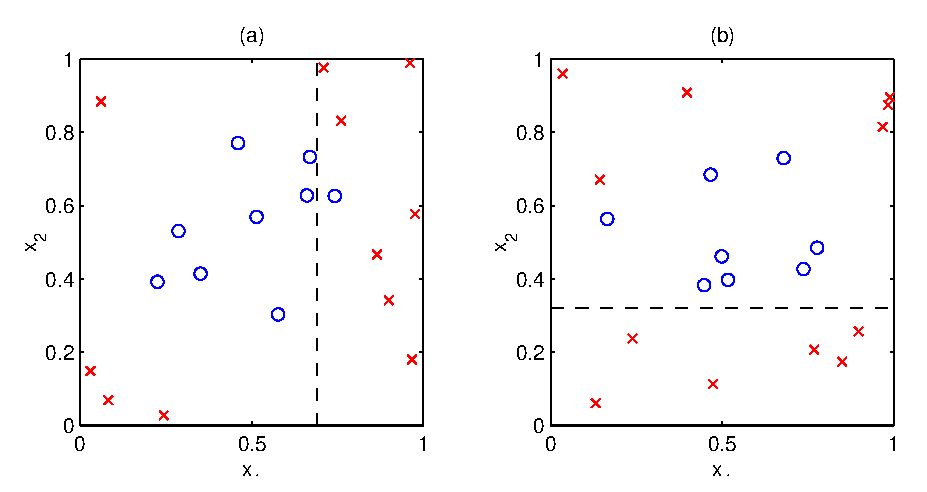
\includegraphics{figures/stumpdiagram.epsg}
\end{center}
\begin{capt}{A decision stump classifier}
Part (a) shows the decision boundary of a decision stump classifier,
and the label of each region.  Part (b) the data it was trained on,
where $\times = -1$ and $\circ = +1$.
\end{capt}
\label{fig:decision stump}
\end{linefigure}

The algorithm constructs a list of possible split locations and
exhaustively searches this list for the minimum of the cost function
(misclassification risk).  Possible split locations are determined by
projecting every data point onto each axis in turn, and bisecting each
pair of consecutive projections to determine the candidate point.  See
figure \ref{fig:candidate points} for a diagram of this process.

\begin{linefigure}
\begin{center}
\includegraphics{figures/stumpcandidates.epsg}
\end{center}
\begin{capt}{Candidate points for decision stump split}
Data points ($\times$) are projected onto the axes.  Each consecutive
pair of projections is then bisected, to generate candidate split
points ($\bullet$).
\end{capt}
\label{fig:candidate points}
\end{linefigure}


\section{Properties of decision stumps}

\begin{theorem}[VC dimension of decision stumps]
\label{theorem:vcdim stumps}
The set $\mathcal{S}$ of decision stump classifiers on an domain
$\calI \subseteq \bbR^d$ has a VC dimension of bounded by 
%
\begin{equation}
\VCdim(\calS) leq d + 1
\end{equation}
%
and, for a dataset of size $m \gg d$ with sufficient variation in its
$\bfx$ parameters, has a constant VC dimension.
%
\proof First part.  Assume that the labels of each branch of the decision
stump are not equal.  Then  our decision boundaries are the set of
axis-orthogonal $d$ dimensional hyperplanes.  This set is contained
within the set of $d$ dimensional hyperplanes (section \ref{sec:vcdim}), so
we know that $\VCdim(\calS) \leq d+1$.

Second part.  We will give a qualitative argument.  In order for the
highest possible VC dimension to be reached, we require that many
split points be available on each axis.  If we have a number of
samples that are ``lined up'' parallel to an axis, then the number of
split points on that axis may be reduced, thereby reducing the VC
dimension.  Thus we require a lot of data that is distributed over
each axis.
\end{theorem}

The important part of this result is that under fairly general
conditions the VC dimension of decision stumps is constant.  This
enables us to make certain assumptions about the complexity of
\emph{combinations} of decision stumps based upon the number of
decision stumps in that combination.

\section{Chapter summary}

We have briefly considered decision stumps, a ``weak'' learning
machine with decision boundaries that are axis orthogonal
hyperplanes.  We have shown how the decision stumps are trained and
that under quite general conditions they have a constant VC dimension.




